\documentclass[letter, 12pt]{article}
\usepackage{color}
\usepackage{verbatim}
\usepackage{enumerate}
\usepackage{caption}
\usepackage{xcolor}
\usepackage{graphicx}
\usepackage{multirow}
\usepackage{subcaption}
\usepackage{amsmath}
 \renewcommand{\labelenumii}{\Roman{enumii}}

\author{Shukti}
\date{\today}
\title{\LaTeX \ sample 2}
\begin{document}
	\maketitle 
	\tableofcontents
\section{Verbatrim}
	\verb|\usepackage{verbatim}|
\section{figure}
\begin{figure}[h]
	\centering
	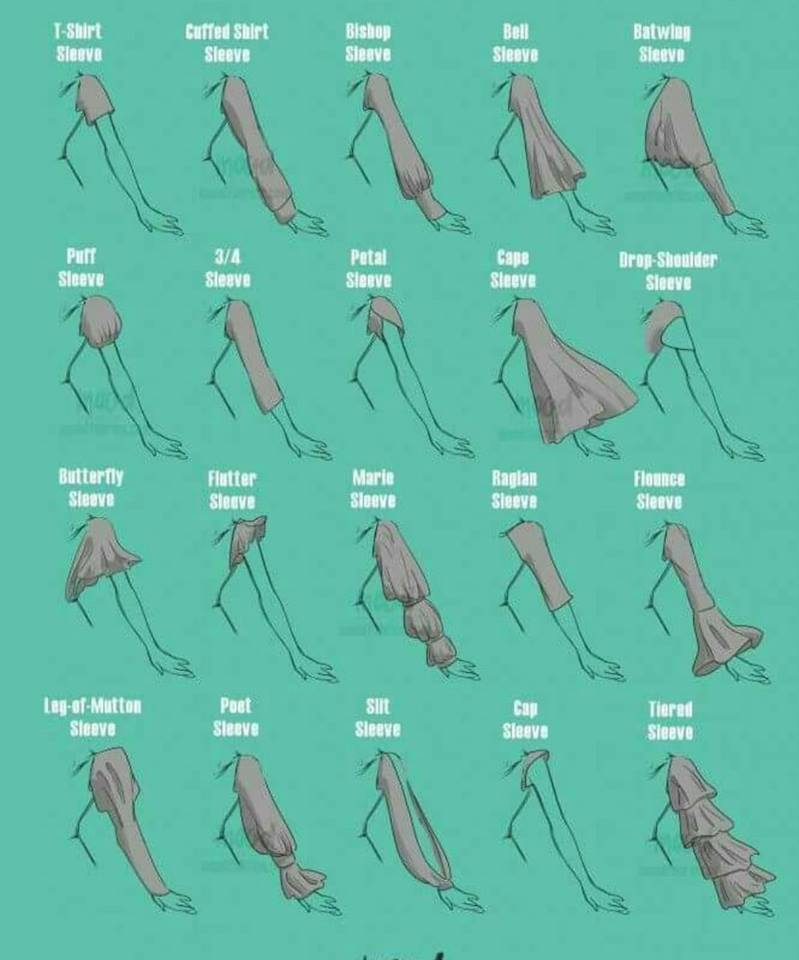
\includegraphics[width=0.3\textwidth]{star.jpg}
	\caption{Sleeve Designs}
	\label{fig:Sleeve}
\end{figure}
\subsection{Subfigure}
\begin{figure}[h]
	\centering
	\begin{subfigure}{.4\textwidth}
		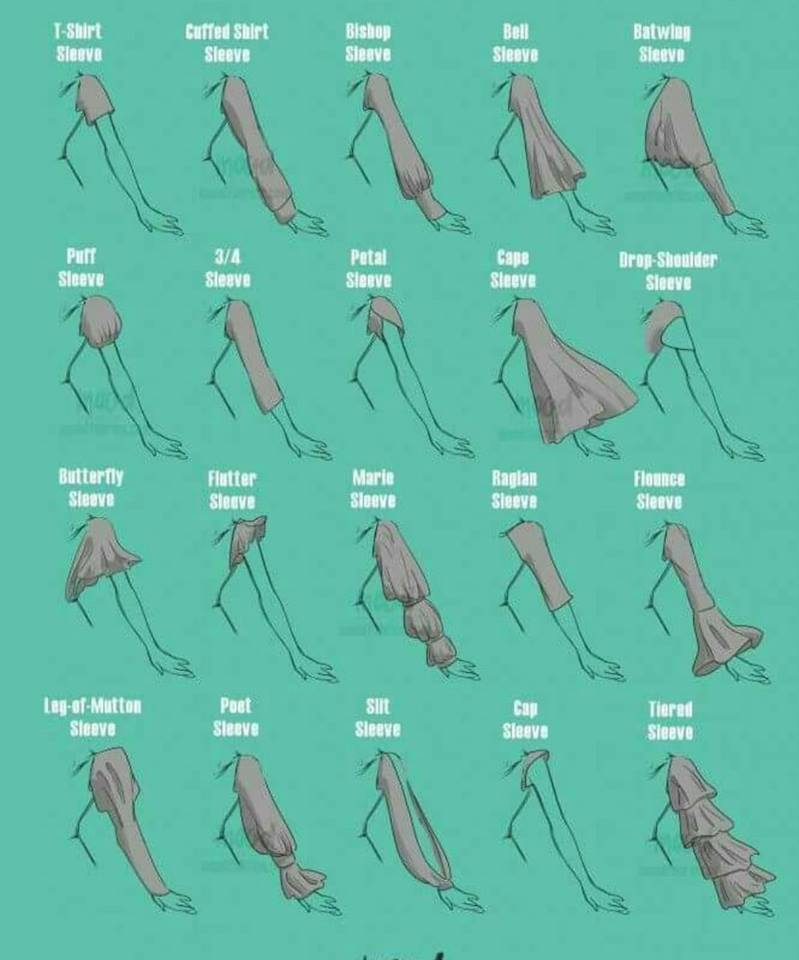
\includegraphics[width=0.8\textwidth]{star.jpg}
		\caption{Sleeve Designs 1}
	\end{subfigure}
	\qquad %will generate gap between pictures
	\begin{subfigure}{.4\textwidth}
		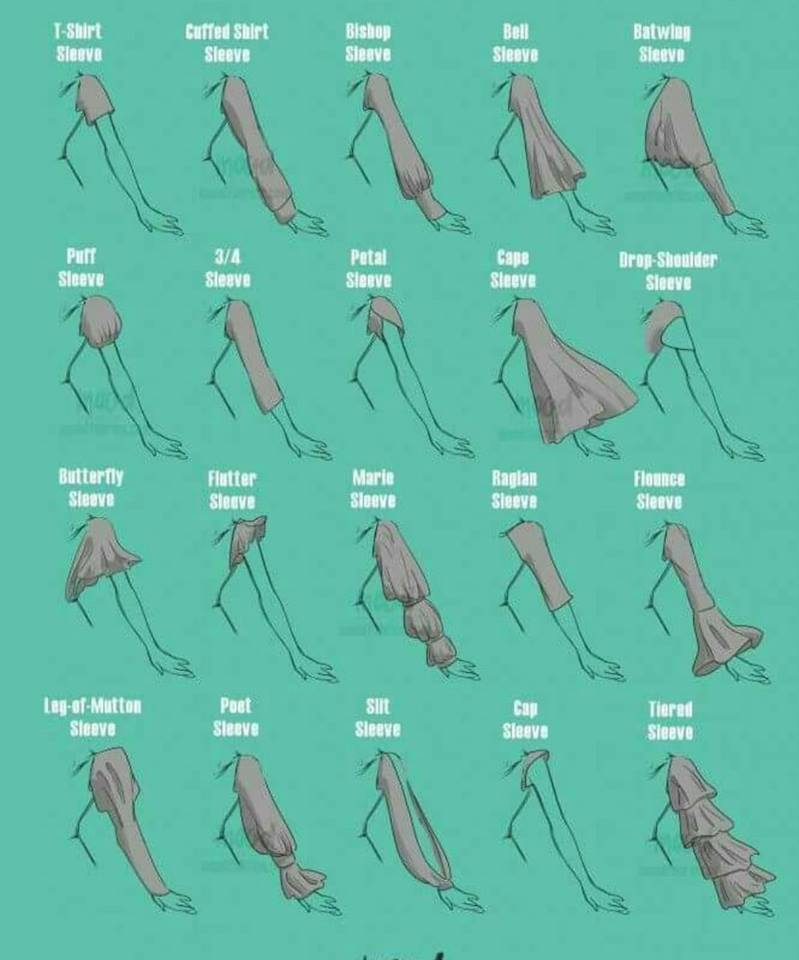
\includegraphics[width=0.8\textwidth]{star.jpg}
		\caption{Sleeve Designs 2}
	\end{subfigure}
	\caption{Sleeve Designs}
\end{figure}
\pagebreak
\section{Bibliography} %also can be hard coded
This book \cite{hochreiter1997long} is amazing.

\bibliographystyle{plain}
\section{Mathmatic Equation}
This is inline $a+a=2a$\\
This is not inline $$a+a=2a$$\\
This is equation \begin{equation}
a_2 \quad +a^{32}=2a
\end{equation}
$$ \int^a_b f(x)dx $$
$$\frac{\tau}{\pi}$$
\begin{equation}
\begin{vmatrix}
1 & 0 & 0 & 1\\
0 & 1 & 0\\
0 & 0 & 1\\
\end{vmatrix}
\end{equation}
\bibliography{bibfile}
\end{document}